\documentclass{beamer}
\usepackage[utf8]{inputenc}
\usetheme{Berlin}
\usecolortheme{wolverine}
\usepackage{amsmath}
\usepackage{listings}
\lstset{
   basicstyle=\fontsize{10}{13}\selectfont\ttfamily
}
%Information to be included in the title page:
\title {Analysis and comparison of matrix vector multiplication codes}
\author % (optional, for multiple authors)
{Ludovico Bessi}
 
\institute[VFU] % (optional)
{
  %
  Matematica per l'ingegneria\\
  Politecnico di Torino
}
\date{May 2019}


\begin{document}
 
\frame{\titlepage}

%Contenuti
\begin{frame}
\frametitle{Table of Contents}
\tableofcontents
\end{frame}

%Prima sezione
\section{Introduction and tools used}
\begin{frame}
\frametitle{Introduction}
\begin{itemize}
 \item Kernel: result[i] = result[i] + A[i,j]$*$vector[j]
 \item Matrix size changing: $n_1 = 40$, $n_2 = 400$, $n_3 = 1000$
 \item Different optimization flags 
 \item What is Eigen? How to change the kernel to match its performance?
\end{itemize}
\end{frame}

\begin{frame}
\frametitle{Tools}
\begin{itemize}
\item  Stream $\to$ Bandwidth 6000 MB/s
\item LIKWID: topology and perfctr
\item Hardware: Interlagos 12-core Opteron processor.
\end{itemize}
\end{frame}

\begin{frame}
\frametitle{Roofline model}
\begin{itemize}
\item  Bottlenecks: CPU bound vs memory bound
\item  $P_{max}$ = $f_{max} * \frac{n_{operations}}{n_{cycles}} * v$
\item  $P = min(P_{max}, \text{Bandwidth} * \text{Computational intensity})$
\end{itemize}




\end{frame}


%Seconda sezione
\section{Different implementations}
\begin{frame}[fragile]
\frametitle{Naive}
\begin{center}
\begin{lstlisting}
       for i = 1:n
       	for j = 1:n 
	  result[i] = result[i] + A[i,j]*v[j]
\end{lstlisting}
\end{center}
\begin{itemize}
\item  Simplest possible code, useful for benchmark.
\item  $P_{max} = \frac{2.6}{8}\frac{Gflops}{s}$, not exploiting pipelines of sum and product
\item  Computational intensity = $\frac{2}{32}\frac{Flops}{Bytes}$
\end{itemize}
\end{frame}
\begin{frame}
\begin{figure}
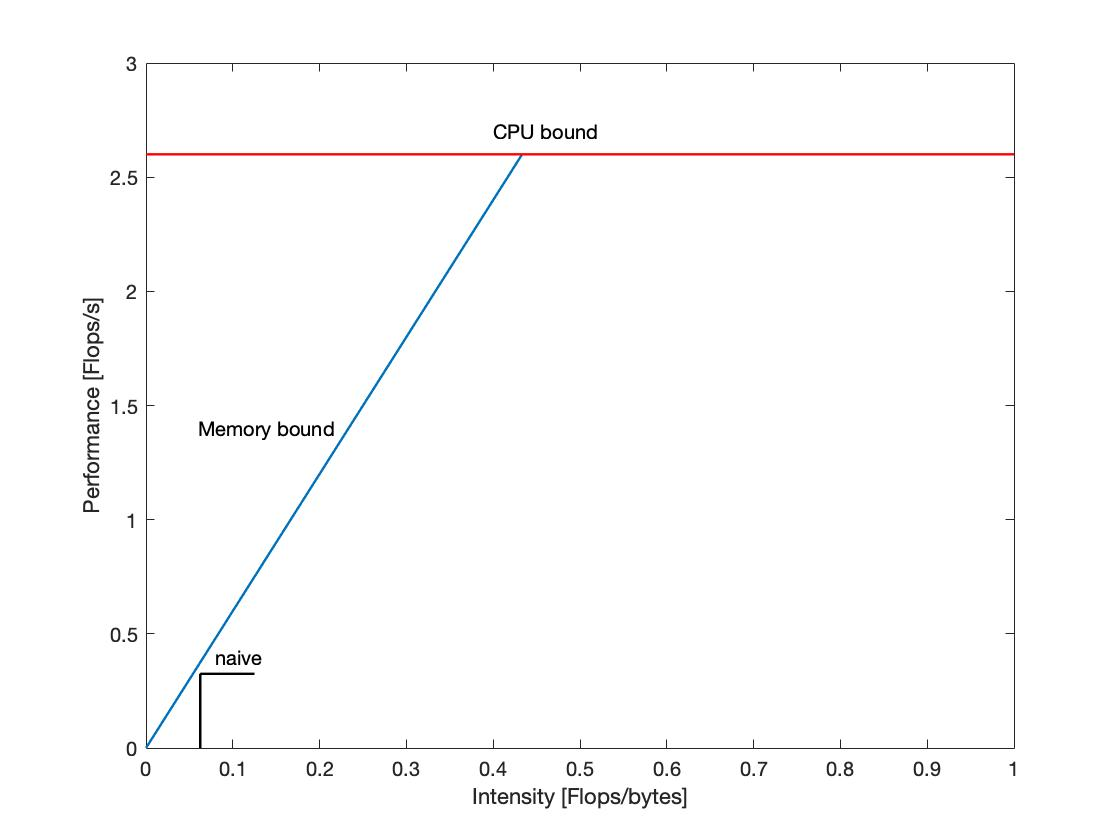
\includegraphics[scale=0.25]{roof_naive}
\end{figure}
\end{frame}

\begin{frame}[fragile]
\frametitle{Temporary variable}
\begin{center}
\begin{lstlisting}
       for i = 1:n
       tmp = result[i]
       	for j = 1:n 
	  tmp = tmp + A[i,j]*v[j]
	result[i] = tmp
\end{lstlisting}
\end{center}
\begin{itemize}
\item Additional temporary variable in outer loop to speed up cache lookup
\item  $P_{max} = \frac{2.6}{8}\frac{Gflops}{s}$
\item Computational intensity = $\frac{2}{16}\frac{Flops}{Bytes}$
\end{itemize}
\end{frame}
\begin{frame}
\begin{figure}
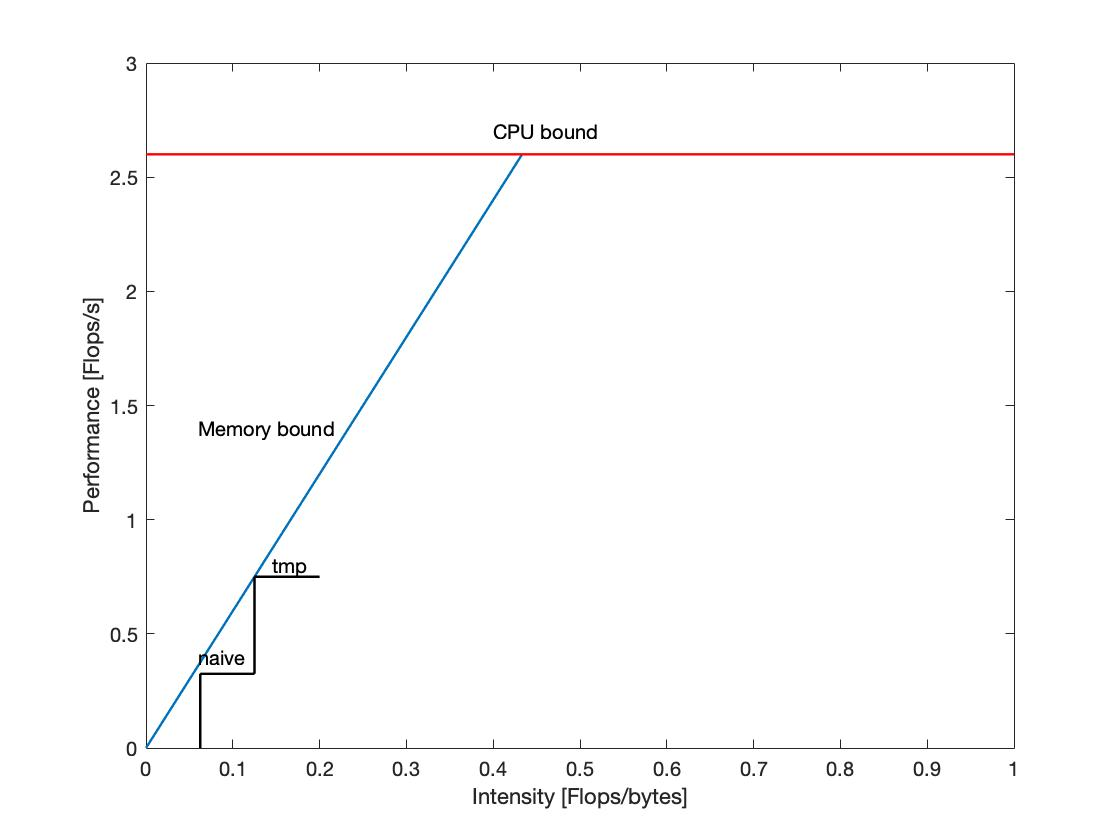
\includegraphics[scale=0.25]{roof_tmp}
\end{figure}
\end{frame}
\begin{frame}
\frametitle{Loop unrolling}
\begin{itemize}
\item Manually split two loops four by four to exploit pipelines of sum and product
\item $P_{max} =2.6\frac{Gflops}{s}$ 
\item Computational intensity = $\frac{32}{160}\frac{Flops}{Bytes}$
\end{itemize}
\end{frame}

\begin{frame}
\begin{figure}
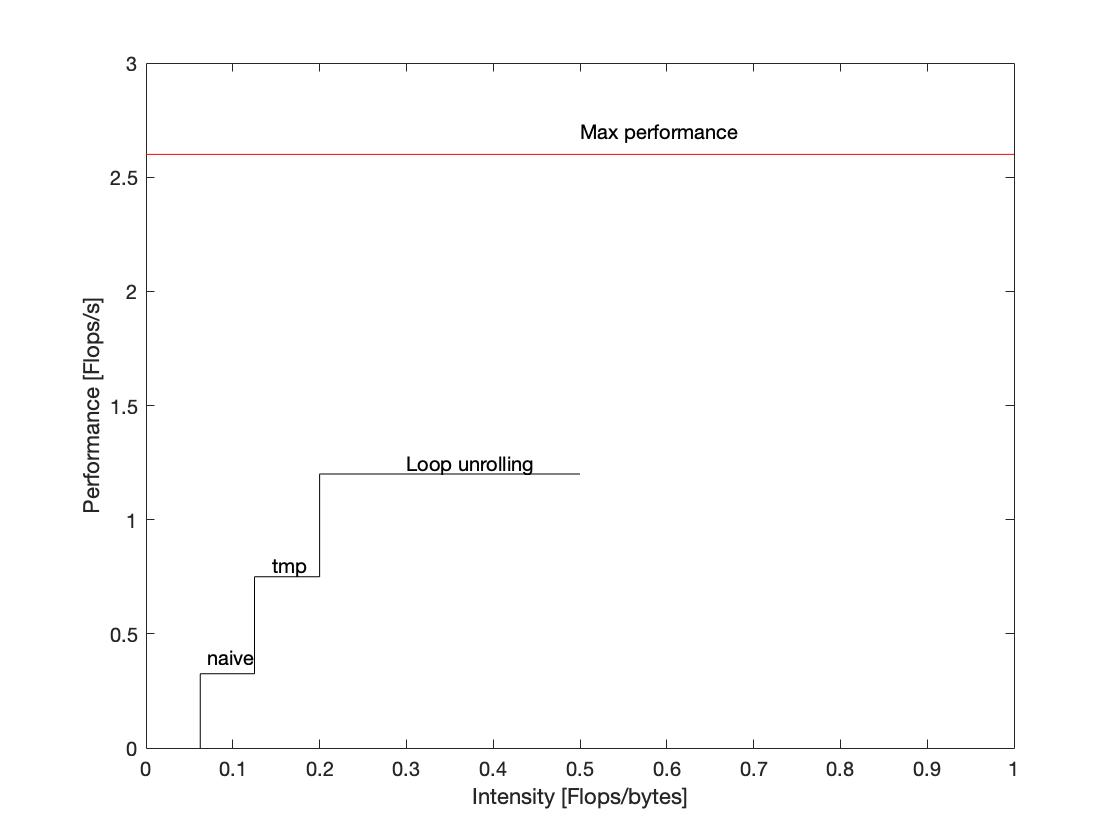
\includegraphics[scale=0.25]{fig_ok}
\end{figure}
\end{frame}

%Terza sezione
\section{Comparison with Eigen}
\begin{frame}
\frametitle{Comparing the Mflops/s}
\begin{center}
\scalebox{0.65}{
 \begin{tabular}{|c c c c c |} 
 \hline
 O0 & naive   & with\_tmp & loop unrolling & eigen \\ [0.5ex] 
 \hline
 n = 40 & 195   & 204       & 313          & 59    \\ 
 \hline
 n = 400 & 328   & 332       & 453                 & 70       \\
 \hline
 n = 1000 & 327  & 328    &  445            & 94   \\
 \hline
\end{tabular}
}
\end{center}


\begin{center}
\scalebox{0.65}{
 \begin{tabular}{|c c c c c |} 
 \hline
 O1 & naive & with\_tmp & loop unrolling & eigen \\ [0.5ex] 
 \hline
 n = 40 & 302 &  255 & 882  & 464\\ 
 \hline
 n = 400 & 948 & 345 & 2346 & 2339\\
 \hline
 n = 1000 & 740 & 344 & 1544 & 1922\\
 \hline
\end{tabular}
}
\end{center}

\begin{center}
\scalebox{0.65}{
 \begin{tabular}{|c c c c c |} 
 \hline
 O2 & naive & with\_tmp & loop unrolling & eigen \\ [0.5ex] 
 \hline
 n = 40 & 313 & 315 & 926  & 455\\ 
 \hline
 n = 400 & 941 & 937 & 3046 & 2297\\
 \hline
 n = 1000 & 720 & 704 & 1523 & 1958\\
 \hline
\end{tabular}
}
\end{center}

\begin{center}
\scalebox{0.65}{
 \begin{tabular}{|c c c c c |} 
 \hline
 O3 & naive & with\_tmp & loop unrolling & eigen \\ [0.5ex] 
 \hline
 n = 40 & 315 & 321 & 915  & 383\\ 
 \hline
 n = 400 & 936 & 961 & 2935 & 3429\\
 \hline
 n = 1000 & 761 & 766 & 1538 & 2024\\
 \hline
\end{tabular}
}
\end{center}
\end{frame}

\begin{frame}
\frametitle{Data visualization}
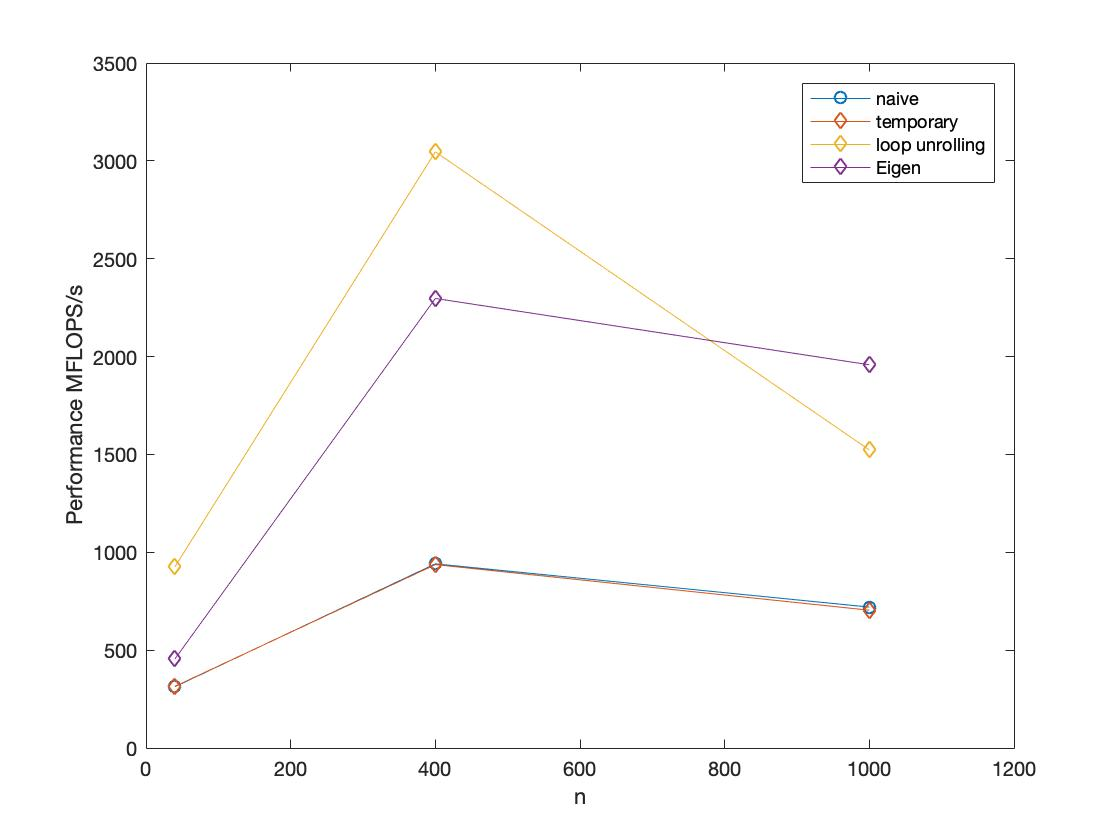
\includegraphics[width=10cm, height=7cm]{plotcolor}
\end{frame}


%Quarta sezione
\section{OpenMP}

\begin{frame}
\frametitle{What is OMP?}
\begin{itemize}
\item API that supports multi-platform shared memory multiprocessing.
\item Used for parallelism within a multi-core node.
\item Based on threads: processes that can share memory.
\end{itemize}
\end{frame}

\begin{frame}
\frametitle{Case study}
With $n = 50000$, $O3$ flag and different number of threads: 
\begin{center}
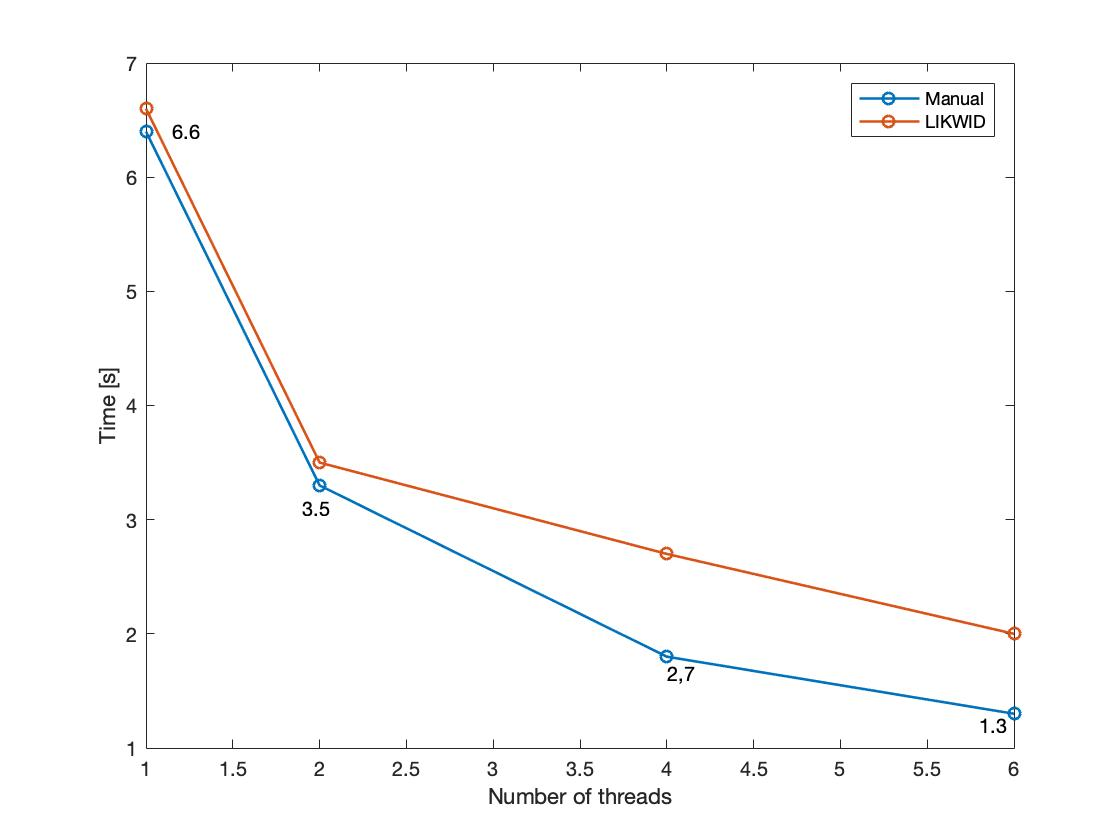
\includegraphics[width=8cm, height=6cm]{graficotimes}
\end{center}
\end{frame}

%Quinta sezione
\section{Conclusions}

\begin{frame}
\frametitle{Achievements}
\begin{itemize}
 \item Outperformed Eigen when $n = 40$
 \item Outperformed Eigen when $n = 400$ and $O2$ flag.
\end{itemize}
 \end{frame}
 
\begin{frame}
\frametitle{Future directions}

\begin{itemize}
 \item Cache aware roof line model
 \item SIMD vectorization
 \item Understanding GCC behaviour when matrix is saved in L1
\end{itemize}
\end{frame}

\end{document}
